\documentclass[tikz,usenames,dvipsnames,margin=3.14mm]{standalone}

\usepackage{pgfplots}
\usepackage{amsmath}
\pgfplotsset{compat=1.17}

\begin{document}
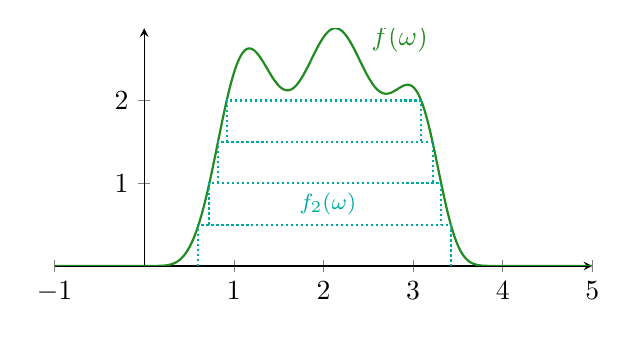
\begin{tikzpicture}
\begin{axis}[scale = .5, 
    domain=-1:5,
    samples=1000,
    % xlabel={\(\Omega \)},
    % ylabel={\(\mathbb R\)},
    legend pos=north west,
    axis lines = middle,
    % xtick = {-10,-8,-6,-4,-2,0,2,4,6,8,10,12,14,16},
    % xticklabels = {-10,-8,-6,-4,-2,0,2,4,6,8,10,12,14,16},
    % ytick = {0.2,0.4,0.6,0.8,1},
    % yticklabels = {0.2,,0.6,0.8,1},
    % clip = false,
    width=6in,
    height=3in,
]
\addplot[ForestGreen, thick] {2.5*exp(-((x-2)^6)/5) * (0.15*cos(deg(6/3.2*pi*x))+1)};

% rectangle 
\draw [Emerald, thick, densely dotted] (0.6, 0.00) -- (0.6, 0.5) -- (3.42, 0.5) -- (3.42, 0.00);
\draw [Emerald, thick, densely dotted] (0.72, 0.50) -- (0.72, 1.0) -- (3.31, 1) -- (3.31, 0.50);
\draw [Emerald, thick, densely dotted] (0.823, 1.00) -- (0.823, 1.5) -- (3.22, 1.5) -- (3.22, 1.00);
\draw [Emerald, thick, densely dotted] (0.92, 1.50) -- (0.92, 2.0) -- (3.09, 2.0) -- (3.09, 1.50);

% label f(\omega) at (3.5, 2.25)
\node [ForestGreen] at (2.85, 2.75) {\(f(\omega)\)};

\node [Emerald] at (2.05, 0.75) {\footnotesize \( f_2(\omega) \)};

\end{axis}
\end{tikzpicture}
\end{document}
